\documentclass[a4paper]{article}

% imoprts

\usepackage{enumitem}
\usepackage{xargs}
\usepackage[pdftex,dvipsnames]{xcolor}
\usepackage[colorinlistoftodos,prependcaption,linecolor=yellow!30,backgroundcolor=yellow!30,bordercolor=yellow!30]{todonotes}

% commands definition

\newcommandx{\warning}[2][1=]{\todo[linecolor=red!30,backgroundcolor=red!30,bordercolor=red!30,#1]{#2}}
\newcommandx{\request}[2][1=]{\todo[linecolor=blue!30,backgroundcolor=blue!30,bordercolor=blue!30,#1]{#2}}
\newcommandx{\info}[2][1=]{\todo[linecolor=green!30,backgroundcolor=green!30,bordercolor=green!30,#1]{#2}}

%------------------------------------------------------------------------------------

\begin{document}

\begin{titlepage}
	\centering
    
    {\normalsize 
        Software Engineering 2 - Prof. Di Nitto Elisabetta \\ 
		Dipartimento di Elettronica, Informazione e Bioingegneria \\
        Politecnico di Milano \par
    }     \vspace{3cm}

    {\Huge \textbf{CLup - Customer Line-up\\} }    \vspace{1cm}
  
    {\large \textbf{RASD\\Requirement Analysis and Specification Document} \par}     \vspace{4cm}

	{\normalsize Andrea Franchini(xxxxxxx) \\ Ian Di Dio Lavore (10580652)\\ Luigi Fusco(xxxxxxxx)\par}     \vspace{3cm}

    
\includegraphics[scale=0.4]{images/logo.pdf}     \vspace{0.5cm}

	{\normalsize xx-xx-2020 \par}
	
\end{titlepage}

\listoftodos

\tableofcontents

    \section{Introduction}\label{sec:intro}

General introduction. \todo{This is a todo}Text.

General introduction. \warning{This is a warning}Text.

General introduction. \request{This is a request}Text.

General introduction. \info{This is an info}Text.

\subsection{Purpose}
This document is the Requirement Analysis and Specification Document for the Customers Line-Up system.
The purpose of this document is to describe the system focusing on scenarios, use cases, requirements and specifications,
analyzing what the software will do, how it will be used and the constraints under which it will operate.
This document is intended both for users and developers.

\subsection{Scope}
\info{here we include an analysis of the world and of the shared phenomena}

\emph{Customers Line-Up} (CLup) is a tool that allows supermarket managers to regulate the influx of people inside
physical stores and aims reduce the time spent by customers waiting in line, especially in emergency lockdown scenarios.
The system allows users to 
This tool reaches the goal by offering a number of functionalities, including:\todo{revise/add more}
\begin{itemize}
    \item access to the service via mobile app or website
    \item physical alternatives for people that do not have Internet access
    \item monitor the amount of people in a store
    \item book a visit, notifying customers of any change in the schedule
    \item suggest alternate stores and/or time frames
    \item track the time spent by customers to estimate waiting times
\end{itemize}

\subsubsection{Current System}
While there are already existing similar services, they are usually indipendent from store chains and
therefore have limited functionalities. CLup is a service that supermarket chains can implement alongside
their existing services. The system is as indipendent as possible from existing infrastructures, and
it can be used with minimal setup.

\subsubsection{Goals}
\begin{enumerate}
    % Users
    \item Allow a User to sign up for an Account after providing a mobile phone number.
    \item Allow a User to book a visit to a specific store.
        \begin{enumerate}
            \item Allow a User to book a visit via Mobile App.
            \item Allow a User to book a visit via Website.
            \item Allow a User to book a visit in a specified time.
            \item Allow a User to book a visit as soon as possible.
        \end{enumerate}
    \item Allow a User to find Stores nearby their current location.
    \item Allow a User to find Stores nearby a specified location.
    \item Allow a User to preview an estimate of the queue time.
    \item Allow a User to cancel their booking.
    \item Allow a User to retrieve a scannable QR Code/Barcode that they must present in order to be granted access to a store.
    \item Allow a User without Internet access to retrive a ticket from a physical location that counts as a booking for a certain time.
    \item Allow a User to book for someone else.
    \item Allow a User to link their Account to the Store Loyalty Program.
        \begin{enumerate}
            \item Users do not have an Account cannot are not entitled to this feature.
        \end{enumerate}
    % Store
    \item The System notifies the Users affected by delay.
    \item The System will postpone Users visits in case of a delay.
    \item The System will not \request{Are we sure about this?}anticipate User visits when a User delete their reservation.
    \item The System must enforce the limits on the allowed number of concurrent Customers inside a store.
        \begin{enumerate}
            \item There can be less Customers than the limit.
            \item There cannot be more Customers than the limit.
            \item The queue is updated each time a Customer exits or enters the store.
        \end{enumerate}
    \item The System will not admit Users that arrive earlier, even if the current number of Customers isn't maximum.
    \item The System will grant a User access only after the User's time of booking.
    \item The System will invalidate a User's booking if they do not show up during a certain time interval.
    \item The System will reserve a certain number of the allowed quote of customers for a special category of Users.
        \begin{enumerate}
            \item The system will grant access to Users without a booking that show up at the store and are pregnant women, elderly or with disabilities.
        \end{enumerate}
    % System Managers
    \item Allow System Managers to set a limit to the people allowed into the store at a time.
    \item Allow System Managers to not provide the physical ticket option.
    \item Allow System Managers to enable the link Account to Loyalty Program feature.
\end{enumerate}

\subsection{Definitions, Acronyms, Abbreviations}

\subsubsection{Definitions}
\begin{itemize}
    \item Customer/User/Visitor: A person that intends to shop at a store.
    \item Registered User: A User that has registered an Account withing the System.
    \item System Manager: An employee of the store chain that can tweak the parameters of the System.
    \item Account: A reference to a specific User in the System, that allows to track the User across multiple visits.
    \item Booking/Reservation: A User securing beforehand their Visit to a specific Store at a specific time.
    \item Visit: The time frame in which the User enters the store, shops and exits.
\end{itemize}

\subsubsection{Acronyms}
\begin{itemize}
    \item RASD: Requirement Analysis and Specification Document.
    \item API: Application Programming Interface
    \item CLup: Customer Line-up
    \item REST: REpresentational State Transfer
\end{itemize}


\subsubsection{Abbreviations}
\begin{itemize}
    \item {[Gn]}: n-goal.
    \item {[Dn]}: n-domain assumption.
    \item {[Rn]}: n-functional requirement.
\end{itemize}

\subsection{Revision History}
\subsection{Reference History}
\begin{itemize}
    \item Problem Specification Document: \todo{Should we upload it?}``Assignment AY 2020-21.pdf''
    \item https://standards.ieee.org/standard/29148-2018.html
\end{itemize}
\subsection{Document Structure}

    
    \section{Overall Description}\label{sec:overall_desc}

\subsection{Product Perspective}

here we include scenarios and further details on the shared
phenomena and a domain model (class diagrams and state charts)

Customers Line-Up is developed for both shop managers and customers.
The intent is to provide functionalities adding value to the interactions between the two.
Managers have access to a website that will help them to avoid large crowds inside and outside their stores, providing them with useful analytics.
Customers may avoid queues by booking visits to stores via website or mobile application, and will be guided in selectiong the best place and time.
Customers must register an account in order to utilize the website or the mobile app.
Customers who do not possess an Internet-connected device may still utilize the service via physical totems outside the stores.

The system will be developed from scratch, giving great flexibility and scalability.
The privacy of the customers will be guaranteed according to the latest privacy related norms.

\subsubsection{Scenarios}
    \begin{enumerate}[label=\Alph*.]
        \item \textbf{Customer with the mobile app arrives in time}\\
            Ian wants to buy groceries to make a cake. Ian uses CLup to get a ticket for the supermarket with the shortest queue in his area.
            The app provides Ian with an estimate on the travel time (by car or by foot) and the time of the reserved slot. 
            Ian arrives at the supermarket in the correct time slot, scans a code generated by the app and is granted access 
            the store. Once he pays for his groceries he scans again his code, so that he can increase the loyalty points associated with his store chain account.

        \item \textbf{Customer with no knowledge on the booking system}\\
            Pino is an elderly man. Pino knows nothing about Smartphones or Computers. Pino needs to buy a cake for his
            nephew's birthday party, so he decides to go to the local supermarket. When he arrives, he notices that the doors of the supermarket
            aren't opening. He reads the sign pointing him to a totem. 
            As soon as he approaches the machine, the machine activates itself an starts speaking with a reassuring voice. 
            The machine allows Pino to book a reservation to enter the store and instructs Pino on how to do so. 
            As soon as the time is up, Pino places his ticket onto the reader beside the door of the store, and he is granted access. 

        \item \textbf{Customer cancels the reservation}\\
            Luigi, after booking a visit to the store, remembers that he had a visit to the dentist at the same time.
            Since Luigi cares about others, he cancels his reservation, freeing up a time slot to be used by other customers.

        \item \textbf{Customer is unable to provide their code}\\
            Andrea books visit and reaches the store in time, but has forgot to charge his phone, which turns off as he pulls it out of his pocket in order to scan his code.
            Andrea goes at the totem, makes a new reservation, and receives a new code and a new time slot.
        \item \textbf{Manager adjusts the number of users allowed without reservation}\\
            Ada is a store manager that notices that most of the customers at her store are elderly and do not make use of the app. She also notices that very few
            customers actually use the app, and the system is reserving too many spots for customers using the app. She navigates to the web panel of the service,
            logs in with her credentials, and navigates to the correct section, then she increase the number of customers allowed without reservation. The system
            automatically decreases the number of customers allowed by booking with the app.
        \end{enumerate}
        \request{Store employee scans ticket at entrance}
\subsection{Product Functions}\todo{fare dettagliato e numerare}
The functions of Customer Line-Up can be clearly divided in two categories, based on the type of the stakeholder that is being addressed.

\subsubsection{Manager functions}
The manager is the owner of the store or store chain that is using the system.
The functions targeted at the manager regard the management of the queue and the knowledge of statistics about the behavior of the clients.
The system will let managers select the type of commercial exercise (whether single store or chain), manage independently every physical store,
select the number of slots dedicated to reservation and the ones dedicated to a classical queue,
as well as to create a high priority queue for special categories of people.
At the same time the system will provide info about the number of people who are currently in a store,
how the number of people changes over time and the average visit length.

\subsubsection{Customer functions}
The customer is the person who visits a store.
The functions targeted at the customer regard the possibility of skipping queues.
The system will let people book visits at specific time slots or queue up at the moment.
If the user is in the queue, they will be updated live with their estimated time of entrance in the store.
If the user has booked a visit, they will be notified immediately if the system realizes that
their visit has become unfeasable and automatically assign a new time or, in the worst case, cancel completely the visit.
The system will offer the possibility of creating an account and of logging in.
Users using their personal accounts will be able to check their past history.

\begin{comment}
\begin{itemize}
    \item Manager:
    \begin{itemize}
        \item monitor the current status of all stores
        \item obtain information on the behavior of customers
        \item adjust the maximum number of customers allowed inside a specific store
    \end{itemize}
    \item Customer:
    \begin{itemize}
        \item account:
        \begin{itemize}
            \item create a new account
            \item delete an owned existing account
            \item show the reservation history
            \item provide all information related to the account, especially
            \begin{itemize}
                \item average visit duration
                \item favorite stores
            \end{itemize}
        \end{itemize}

        \item booking:
        \begin{itemize}
            \item book a visit to the store
            \item give suggestions regarding when and where to book
            \item send notifications regarding the status of a reservation, whether it has been delayed or deleted
            \begin{itemize}
                \item send notifications via mobile app
                \item send notifications via SMS
                \item send notifications via phone call
            \end{itemize}
            \item cancel a reservation
        \end{itemize}

        \item show nearby stores and their availability
    \end{itemize}
\end{itemize}
\end{comment}

\subsection{User Characteristics}
Customers Line-Up is mainly aimed at essential and widely used services.
Because of this its audience will be wide and diversified, and the system will be easy to use and accessible in several of ways, accounting in particular for people with disabilities or people who are not familiar with technology.
On one side of the system there is the system manager (single or multiple), who will monitor how the system is used and obtain useful information.
They are usually already familiar with othe customer relationship managers and already know what to expext from a control panel.
On the other side there is the customer, who uses the system in order to avoid boring lines and to prevent contact with others.
The main categories of customer are:
\begin{itemize}
    \item \textbf{Tech-friendly}\\
        People who are familiar with modern technologies. They find it easy to navigate the menus of a complex application.
        They are able to use the system in an autonomous way and are the ones who will benefit the most from the more complex and advanced features.
    \item \textbf{Tech-unfriendly}\\
        People who are not familiar with modern technologies. They have problems navigating complex application, and are more accustomed to talking to humans.
        They might need aid using the system or misuse the system. They benefit from a system designed around clarity and simplicity, or from different, easier ways of using the system.
        This category includes people with disabilities.
\end{itemize}

The objective of Customers Line-Up is to be as inclusive as possible, providing utilities targeted at all possible users.

\subsection{Assumptions, Dependencies, and Constraints}

\subsubsection{Domain Assumptions}
\begin{enumerate}[label={[D\arabic*]}]
    \item The number of people in a store cannot go over a certain fixed amount
    \item If an user enters the store they will exit the store before it closes
    \item \todo{Dobbiamo mettere che ci sono i tornelli o c'è una persona}The system reliably counts the number of people entering and exiting the store
    \item The time of real operation of the store corresponds with the one registered in the system
    \item A customer cannot enter the store without using the system
    \item External software dependencies the system relies on always provide true data and never fail
\end{enumerate}

\subsubsection{Dependencies}
\begin{itemize}
    \item The system requires access to a third party maps API.
    \item The system needs a third party API in order to send SMS to customers' phones.
    \item The mobile app shall be deployed on major mobile phones operating systems (Android, iOS).
    \item The website requires a modern browser (no legacy browser support).
    \item The application deployed on the totem has to be compatible with its operative system. \warning{maybe it should be the web app?}
\end{itemize}

\subsubsection{Constraints}
\begin{itemize}
    \item The system shall be compliant to local laws and regulations, in particular users data should
    be treated according to the \href{https://gdpr.eu/}{GDPR}. This means that users should be always able
    to request their data.
    \item The system should in first place limit itself to collect only
    the necessary ones to function, such as the user telephone number.
    \item To better protect the users' sensitive information, such as their telephone number, their data should
    be encrypted.
\end{itemize}

    \section{Specific Requirements}\label{sec:spec_req}

Here we include more details on all aspects in Section 2 if they
can be useful for the development team. 

\subsection{External Interface Requirements}
\subsubsection{User Interfaces}

The application is designed to allow the customer to make a reservation for a certain hour
or to register in the current queue of a supermarket. The first time the user opens the app,
they are prompted to register for an account: they have to provide their mobile phone number
(Fig. \ref{fig:mockup-welcome}), then they'll receive an SMS with a confirmation code
(Fig. \ref{fig:mockup-login}) to insert.
If the code inserted is the one sent to the phone number inserted in the first screen, the
account creation is successful.

If the registration is successful, the user can immediately see a map (Fig \ref{fig:select-store})
with stores nearby their location (they might have to allow the app do receive their location through
the OS API), otherwise they can manually search stores by typing an address.
Stores are also listed by distance and queue length.

Upon selecting a store (Fig. \ref{fig:store-details}), the current number of people in queue is shown to the user,
as well as the estimated waiting time in queue. They can choose to enter the queue as soon as
possible, or to pick an available time slot.

If they choose to pick a time slot, they are shown a list of time slots sorted by day (Fig. \ref{fig:select-timeslot}).
Upon confirmation, the user receive a receipt (Fig. \ref{fig:receipt}) with the date and time of their reservation,
and a QR code that they'll need to show when they present themselves at the store.

Should the customer queue for the first available time slot, then they will receive a similar receipt (Fig. \ref{fig:queue-ticket}),
that has a countdown of the time remaining in queue before their visit.

\begin{figure}[h]
    \caption{Mock-up of the Application User Interface}
    \subfloat[Welcome Screen]{
        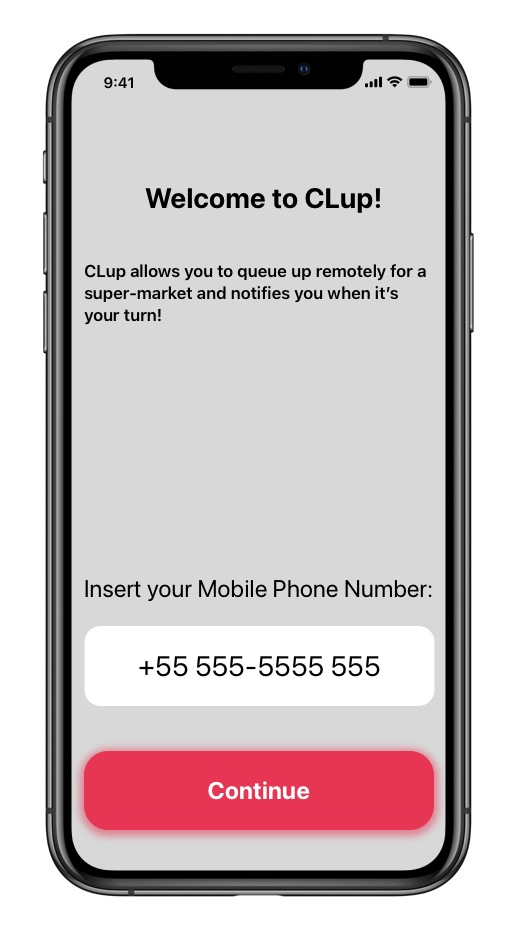
\includegraphics[width=0.25\textwidth]{images/mockup/welcome-screen.png}
        \label{fig:mockup-welcome}
    }
    \subfloat[Confirm Login]{
        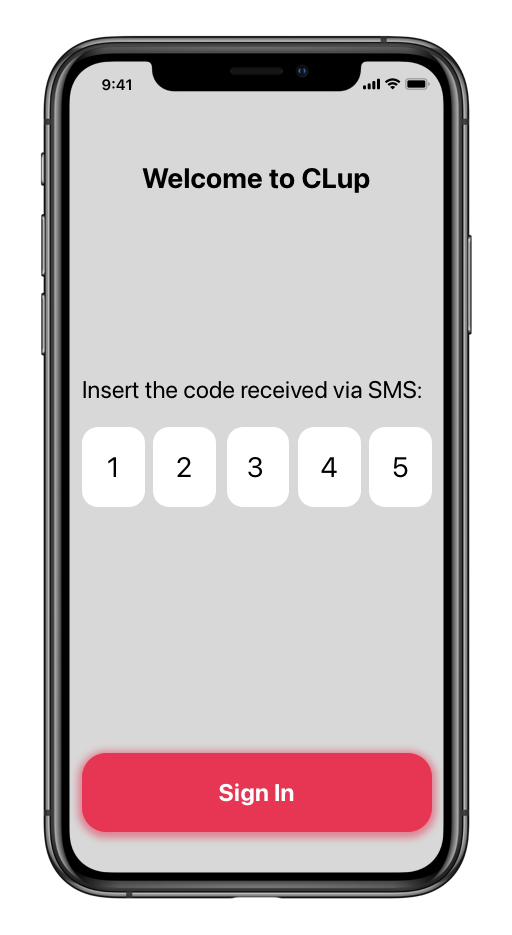
\includegraphics[width=0.25\textwidth]{images/mockup/confirm-login.png}
        \label{fig:mockup-login}
    }
    \subfloat[Select Store]{
        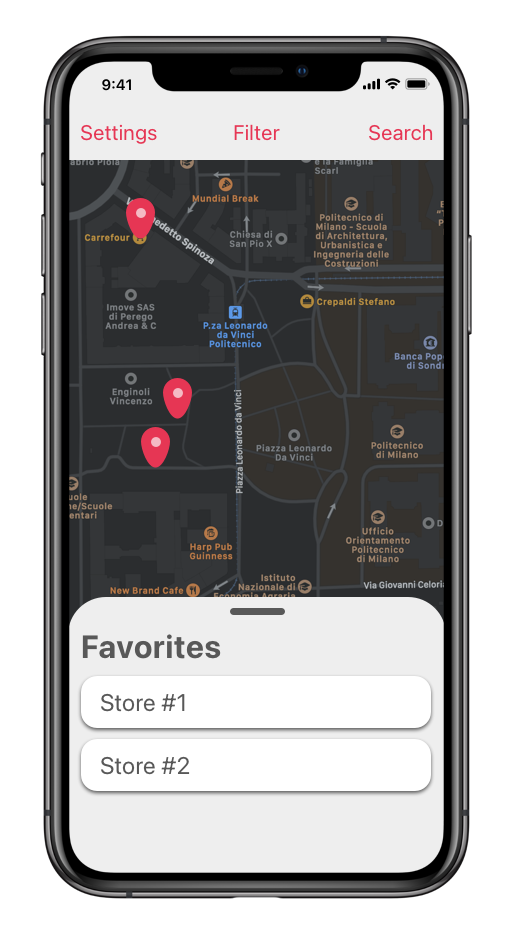
\includegraphics[width=0.25\textwidth]{images/mockup/map-select.png}
        \label{fig:select-store}
    }
    \subfloat[Store Details]{
        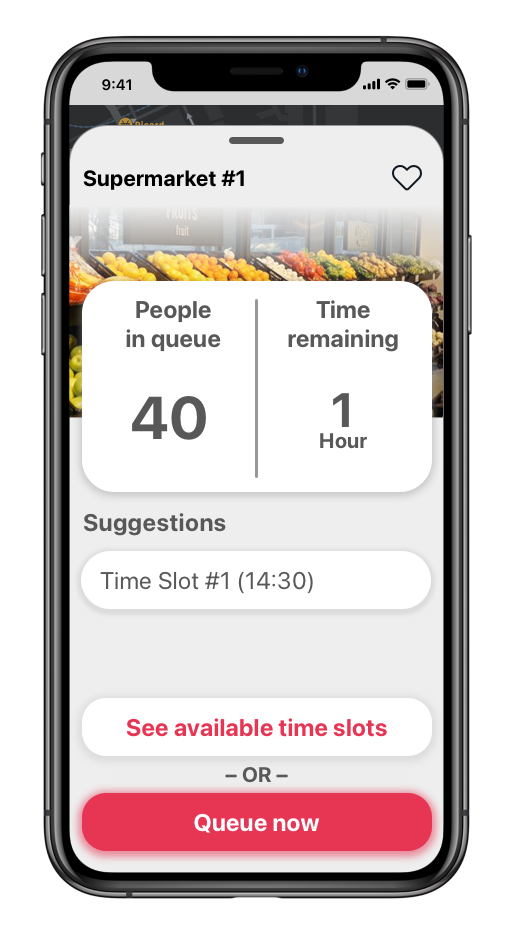
\includegraphics[width=0.25\textwidth]{images/mockup/store-detail.png}
        \label{fig:store-details}
    }
    \newline
    \subfloat[Select Timeslot]{
        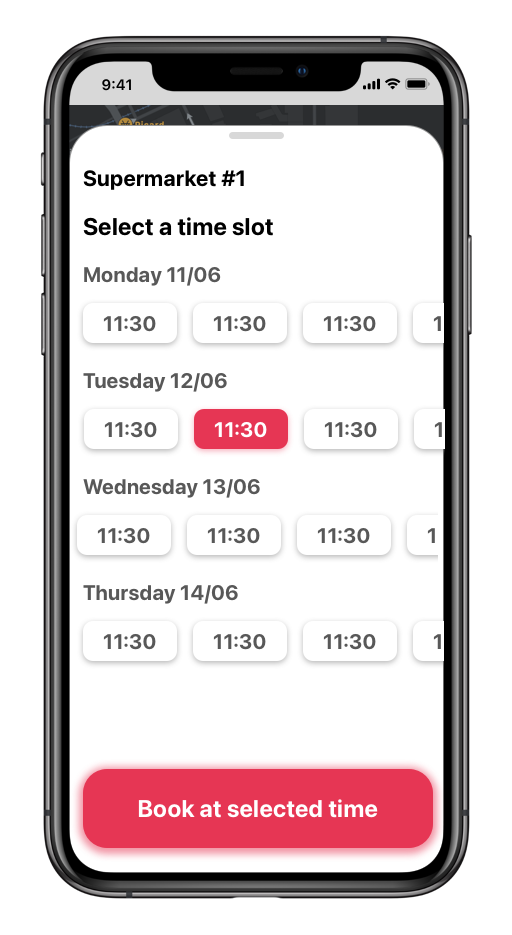
\includegraphics[width=0.25\textwidth]{images/mockup/time-slots.png}
        \label{fig:select-timeslot}
    }
    \subfloat[Reservation Receipt]{
        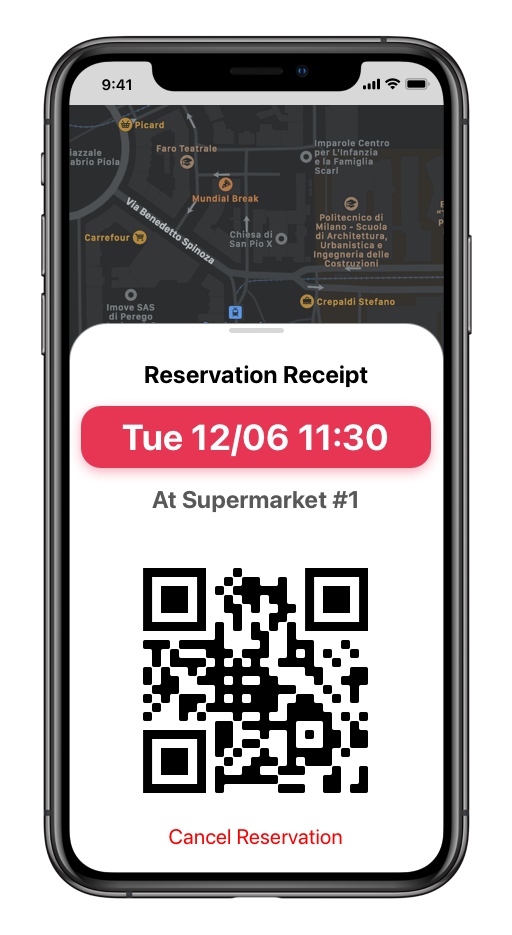
\includegraphics[width=0.25\textwidth]{images/mockup/receipt.png}
        \label{fig:receipt}
    }
    \subfloat[Queue Ticket]{
        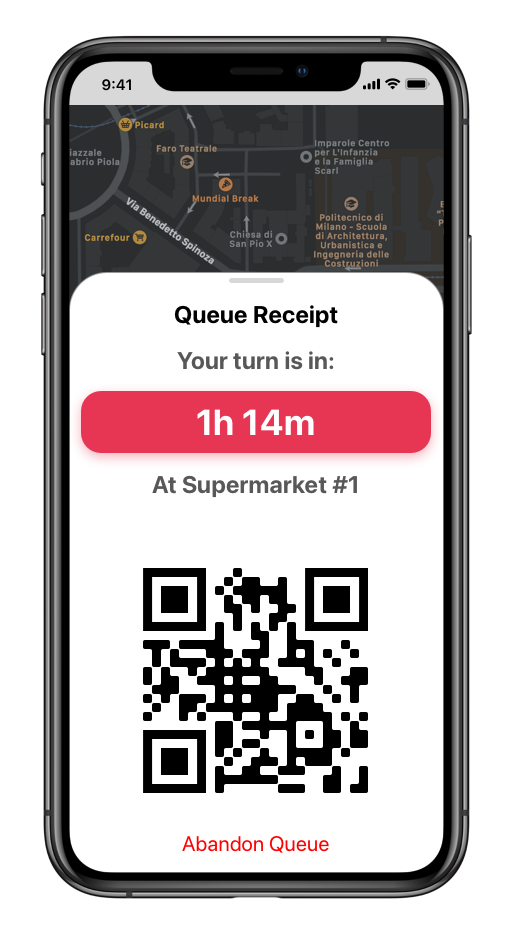
\includegraphics[width=0.25\textwidth]{images/mockup/queue-ticket.png}
        \label{fig:queue-ticket}
    }
\end{figure}


\subsubsection{Hardware Interfaces}

To account for Customers without an Internet-connected device,
an interactive totem (Fig. \ref{fig:totem}) with a touchscreen display should be made available at each store entrance.
The totem is connected to Internet or the store local network.
It mirrors the key features of the web application, but it doesn't require the customer to
authenticate. Customers may reserve a time-slot, or enter the queue, but they won't be able to
be notified of possible changes. The reservation receipt is printed and the customer must keep it until they're
admitted to the store, otherwise they won't be able to enter.
\begin{figure}[h]
    \centering
    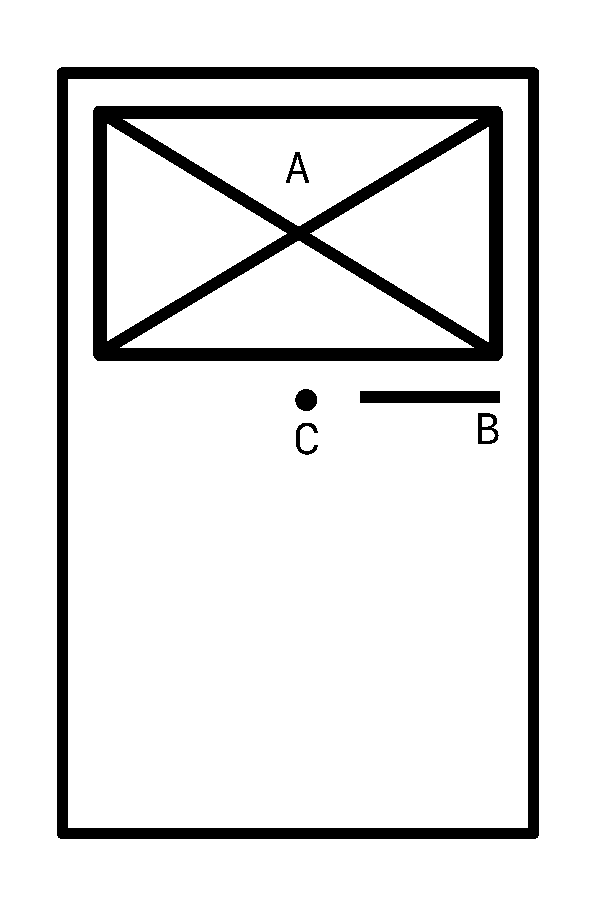
\includegraphics[width=0.25\textwidth]{images/totem.pdf}
    \caption{The totem interface: (A) is the touchscreen display,
    (B) is where the printed ticket is emitted, (C) is a proximity sensor that wakes the
    totem when a client is nearby.}
    \label{fig:totem}
\end{figure}

\subsubsection{Software Interfaces}
\subsubsection{Communication Interfaces}

\subsection{Functional Requirements}
Definition of use case diagrams, use cases and associated
sequence/activity diagrams, and mapping on requirements

\begin{enumerate}[label={[R\arabic*]}]
    % Users
    \item Allow a User to find Stores nearby a specified location.
    \item Allow a User to get in the virtual line.
    \item Allow a User to preview an estimate of the queue time.
    \item Allow a User to cancel their reservation.
    \item Allow a User to retrieve a scannable QR Code/Barcode that they must present in order to be granted access to a store.
    \item Allow a User to sign up for an Account after providing a mobile phone number.
    \item Allow a registered User to book a visit for themselves or for someone else to a specific store.

    % Store
    \item The System notifies the Users affected by delay.
    \item The System postpones Users visits in case of a delay.
    \item The System enforces the limits on the allowed number of concurrent Customers inside a store.
    \item The System does not admit Users that arrive earlier, even if the current number of Customers isn't maximum.
    \item The System grants a User access only after the User's time of reservation.
    \item The System invalidates a User's reservation if they do not show up during a certain time interval.
    \item The System reserves a certain number of the allowed quote of customers for a special category of Users.
    \item The system grants priority access to Users without a reservation that show up at the store and are pregnant women, elderly or with disabilities.
    
    % System Managers
    \item Allow System Managers to set a limit to the people allowed into the store at a time.
    \item Allow System Managers to not provide the physical ticket option.
    \item Allow System Managers to enable the functionality that allows customers to link their Account with Loyalty Program feature.
\end{enumerate}

\begin{center}
    \begin{tabular}{ |c||c|c| }
        \hline
        \textbf{Goal} & \textbf{Requirements} & \textbf{Assumptions} \\
        \hline
        G1 & R1, R2, R3, R4, R5, R6 & \\
        \hline
        G2 & R3, R7, R8, & \\
        \hline
        G3 & R5, R10 & \\
        \hline
        G4 & & \\
        \hline
        G5 & & \\
        \hline
    \end{tabular}
\end{center}




%----------------------------------------------------------------------------------------------------
%                                           USE CASES
%----------------------------------------------------------------------------------------------------

%LOGIN
\usecase
{Sign Up}
{Customer}
{The Customer has installed the application on their device.}
{
    \begin{enumerate}
        \item The Customer opens the application.
        \item The Customer may read Privacy Policy and the Terms of Service by clicking on the respective links. If they create an account, it's implied that they accept them.
        \item The Customer enters their mobile phone number and taps ``Continue''.
        \item The Customer enters the received code via SMS and taps ``Sign In''.
    \end{enumerate}
}
{The Customer is now logged-in and they may utilize the application.}
{
    \begin{itemize}
        \item The Customer inputs invalid data.
        \item The Customer doesn't fill the required data.
    \end{itemize}
}
{
    When an exception occurs, the user is informed by a human-readable message.
}


%Join Line
\usecase
{Join Line}
{Authenticated User}
{Authenticated User selects a Supermarket in the application}
{
        \begin{enumerate}
            \item The Authenticated User pushes the "Queue Now" button.
            \item The system provides the Queue Receipt with the generated QR code and the estimated time remaining.
        \end{enumerate}
}
{
    The customer is now in the queue waiting for their turn.
}
{
    \begin{itemize}
        \item There is a major delay in the store. 
        \item The time remaining to wait in the queue exeeds the opening hours of the store. 
    \end{itemize}
}
{
    When an exception occurs, the user has the possibility to remain in the queue or leave it. 
}


%Check Status
\usecase
{Check Status}
{Authenticated User}
{Authenticated User logs-in in the application}
{
        \begin{enumerate}
            \item The System provides the user a list of the supermarkets near him.
            \item The Authenticated User is able to see a preview of the number of people in queue and the estimated waiting time. 
            \item The user selects the desired store. 
            \item The user is now able to see full screen the waiting time and the number of people in queue (and possibly other stats on the store).  
        \end{enumerate}
}
{
    The Authenticated User gain the knowledge on the waiting times and the number of people in queue in the stores near him/her. 
}
{
    \begin{itemize}
        \item There are no open stores in the area. 
        \item There are no stores in the area. 
    \end{itemize}
}
{
    When an exception occurs the users is promted to check the application again later or change the search area. 
}




\subsection{Performance Requirements}
\subsection{Design Constraints}
\subsubsection{Standards Compliance}
\subsubsection{Hardware Limitations}
\subsubsection{Any Other Constraint}
\subsection{Software System Attributes}
\subsubsection{Reliability}
\subsubsection{Availability}
\subsubsection{Security}
\subsubsection{Maintainability}
\subsubsection{Portability}

    
\end{document}
